\begin{TOP}{Netzwerke}
\vspace*{-1.5\baselineskip}
\begin{itemize}
	\item Zeichnungskonventionen\\
		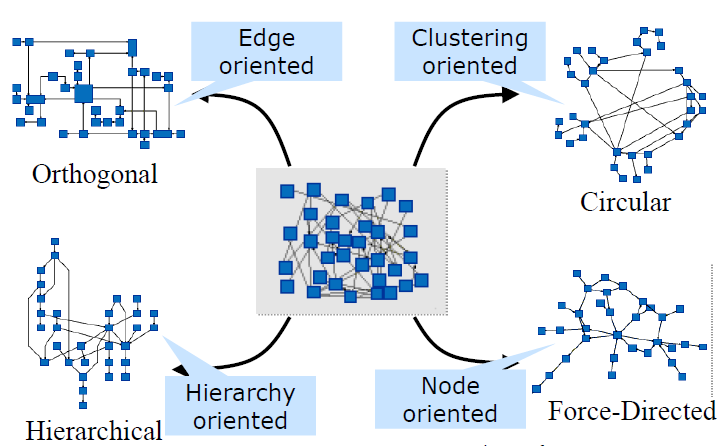
\includegraphics[width=0.8\textwidth]{Pics/05-00-Konventionen.png}
	\item Force-Directed Methoden (Spring Embedder)
		\begin{itemize}
			\item Minimierung von Kantenkreuzungen
			\item Minimierung der Gesamtlänge aller Kanten
			\item maximale Kantenlänge einhalten
			\item einheitliche Kantenlänge einhalten
			\item Minimierung der Kantenknicke
			\item Minimierung von unterschiedlichen Winkeln/Krümmungen
			\item Maximierung der Winkel zwischen zwei Kanten
			\item Minimierung der Gesamtfläche der Zeichnung
			\item Aspect Ratio einhalten
			\item symmetrische Struktur
		\end{itemize}
	\item hierarchisches Kantenbündeln
	\item NodeTrix: hybride Matrix Repräsentation (Matrizen als Knoten)
\end{itemize}
\ \\
\loadTop{05/01-Treemap}
\end{TOP}